
\subsection{Access semantics and optimization goals}
\sys\ is a persistent ordered key-value store. Similarly to popular industrial ones~\cite{hbase,leveldb,RocksDB}, 
it supports concurrent access by multiple threads and ensures strong consistency. 
Specifically its \emph{put, get}, and \emph{scan} operations are \emph{atomic}.  
For scans, this means that all key-value pairs returned by a single scan belong to a consistent 
snapshot reflecting the state of the data store at a unique point in time.

\sys\ persists data to disk to allow it to survive crashes.
%Following a crash, \sys\ recovers to a consistent state reflecting an execution point before the crash.
As in other systems~\cite{leveldb,RocksDB},  it supports
\emph{asynchronous} persistence, where puts are buffered before being persisted in the background,  
 trading durability for speed. In this case, some recent updates may be lost but 
 recovery is to a \emph{consistent} state  in the sense that 
if some put is lost, then no ensuing (and thus possibly dependent) puts are reflected.


\noindent
Our key optimization goals are the following:
\begin{enumerate}
%\itemsep0pt
\item Optimize for {spatial locality}, e.g., workloads that employ composite keys.
\remove{
 Many NoSQL applications embed multi-dimensional data in a single-dimension composite key. 
 This design provides high spatial locality on the primary dimension (key prefix). We strive
 to express this locality in physical data organization.
 }
 
\item Minimize {write amplification}  to reduce disk wear.%, especially for SSD devices.
 
\item %{\bf High performance  with memory-resident working sets.}
%To sustain high speed, key-value stores nowadays leverage increasing RAM sizes where they can hold most of the active working set. 
Strive for high performance in  \emph{sliding-local} scenarios, where most of the active working set fits in DRAM. 
Note that we do \emph{not} expect the entire database to fit in
memory, only the active data.  
 
\item Ensure {fast recovery} to a consistent state.  
%Because crashes are inevitable, recovery must ensure consistency and the downtime it entails should be kept  short. 
\end{enumerate}

\subsection{Design choices}

\sys\ combines the spatial locality of B-trees with the optimized I/O and quick access of LSMs. 
Its data layout is illustrated in Figure~\ref{fig:piwi}.  We now discuss its key components.   

\begin{figure}[tb]
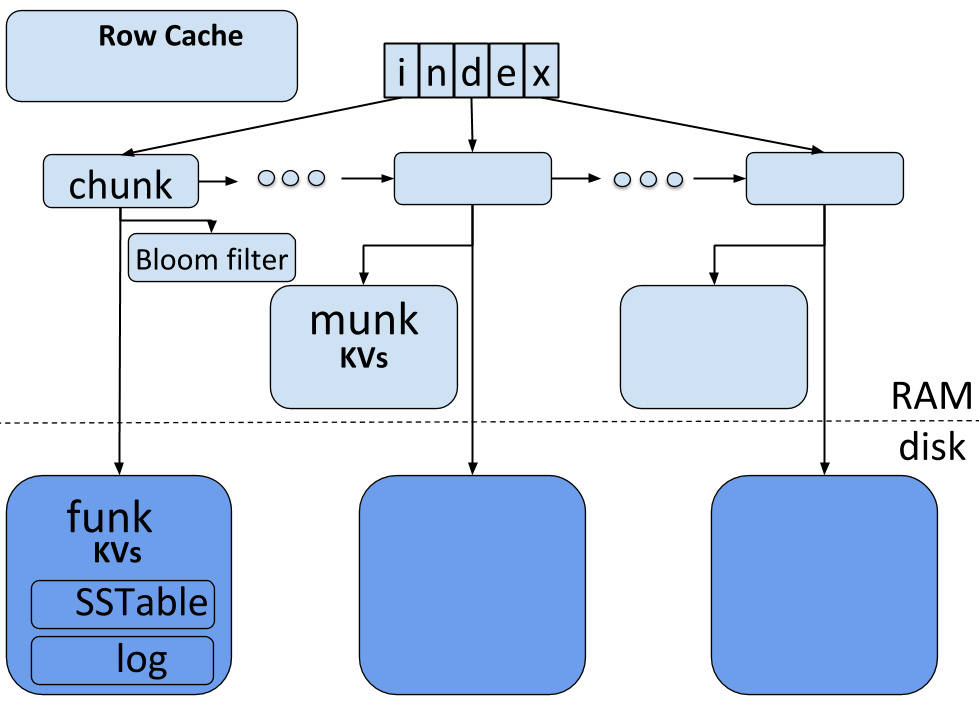
\includegraphics[width=\columnwidth]{PiWi.png}
\caption{\sys's  organization. Gray boxes depict metadata, light blue areas show RAM caches of KV-pairs, and blue areas represent on-disk KV storage.}
\label{fig:piwi}
\end{figure}


{\bf Chunks.\ }
To leverage spatial locality, we partition data -- both on-disk and in-memory -- by key.
Our  data structure is organized as a 
%sorted linked 
list of \emph{chunks} holding consecutive key ranges. 
All chunks are represented in memory via lightweight volatile metadata objects, which are reconstructed from disk on recovery.

{\bf Sequential I/O with in-chunk logging.\ }
For persistence, each chunk has a file representation called  \emph{funk} (file chunk), which holds all the KV-pairs in the chunk's range.
Within funks, we adopt LSM's sequential I/O approach. To this end, the funk 
is divided into two parts: (1) a sorted \emph{SSTable} (Sorted String Table~\cite{Bigtable2008}), and (2) an unsorted \emph{log}. 
New updates are appended to the log; the log is  merged into the SSTable via an infrequent background compaction process. 
Under spatial locality,  popular logs are targeted frequently, allowing effective batching. 
Unlike LSMs, \sys\ logs writes exclusively within their funks and avoids duplicating the updates  in a separate WAL. This reduces write amplification and expedites recovery. 

{\bf Chunk-level caching with in-memory compaction.\ }
DRAM caches are instrumental for read performance. 
To favor workloads with spatial locality, we cache entire chunks:
a popular chunk is cached in a  memory data structure called \emph{munk} (memory chunk).
Like their on-disk counterparts, munks have a compacted sorted prefix while new updates are appended at the end and remain unsorted until the next compaction. 
Whereas LSM caches  only serve the read-path, the chunk granularity allows us to 
leverage munks also in the write-path, specifically, for in-memory compaction.  
We observe that 
%Whereas appending writes to the log is essential for persistence, 
compacting a funk's log is only required for performance (to expedite on-disk lookup) and is redundant when the chunk is cached. Thus, when 
a chunk has a munk, we compact it almost exclusively in memory and allow the disk log to grow. 
Note that if a chunk does not have a munk, it usually means that the chunk is ``cold'' 
and hence there is little or no new data to compact. So either way, disk compaction is rare, and write amplification is low.

{\bf Fast in-memory access.\ }
Chunks are organized in a sorted linked list. To speed up lookups, they are indexed using a volatile index (a sorted array in our implementation).  

 
 {\bf Row caches and Bloom filters.\ }
 \sys\ adopts two standard mechanisms from LSMs. First, to expedite access to  keys whose chunks are only on-disk  (i.e., have no munks), 
a \emph{row cache} of individual popular keys serves the read-path. The row cache is important for workloads that lack
spatial locality where caching an entire chunk for a single ``hot'' key is wasteful. 
Second, for munk-less chunks, we employ \emph{Bloom filters} to limit excessive access to disk. 

{\bf Concurrency and multi-versioning.\ }
 \sys\ allows high parallelism among threads invoking its API calls. 
 Read operations are wait-free (never block) and puts use lightweight synchronization. 
 To support atomic scans, we  employ a light form of multi-versioning that uses 
copy-on-write to keep old versions only if they may be required by ongoing scans. 
In other words, if a put attempts to overwrite a key required by an active scan, then a new version is created alongside the 
existing one, whereas versions that are not needed by any scan are not retained. 
Thus, version management incurs a low overhead (as it occurs only on scans). 
%It also defines a simple rule for garbage collecting old versions.
In addition, tagging each value with a version allows \sys\ to easily recover to a consistent point in time, namely a version below which all puts have been persisted to disk.


